\documentclass[xetex,12pt,compress,hyperref={xetex}]{beamer}
\usetheme{Warsaw}% есть много тем, может поробовать ещё CambridgeUS, Boadila, Goettingen, Hannover, Szeged
\usefonttheme{serif}
\usepackage{fontspec}
\usepackage{xunicode}
\usepackage{unicode-math}
\usepackage{xltxtra}

\usepackage{polyglossia}
\setdefaultlanguage[spelling=modern]{russian}
\setotherlanguage{english} 

\defaultfontfeatures{Scale = MatchLowercase,Ligatures=TeX}  %% устанавливает поведение шрифтов по умолчанию  
\setmainfont{XITS}
\setmathfont{XITS Math}
\newfontfamily\cyrillicfont{XITS}

\author{Фамилия~И.~О.}
\title{Главное название}
\subtitle{побочное название}
\date{16 мая 2014}

\begin{document}

 \begin{frame}
  \titlepage
 \end{frame}
 
 \section{Введение}
 
 \begin{frame}{Цель и задача}
  Цель: долететь до луны
  \begin{itemize}
    \item задача A
    \item задача B1
    \item задача B2
    \item задача C
  \end{itemize}
 \end{frame}
 
 \begin{frame}{Картинка} 
   \begin{center}
    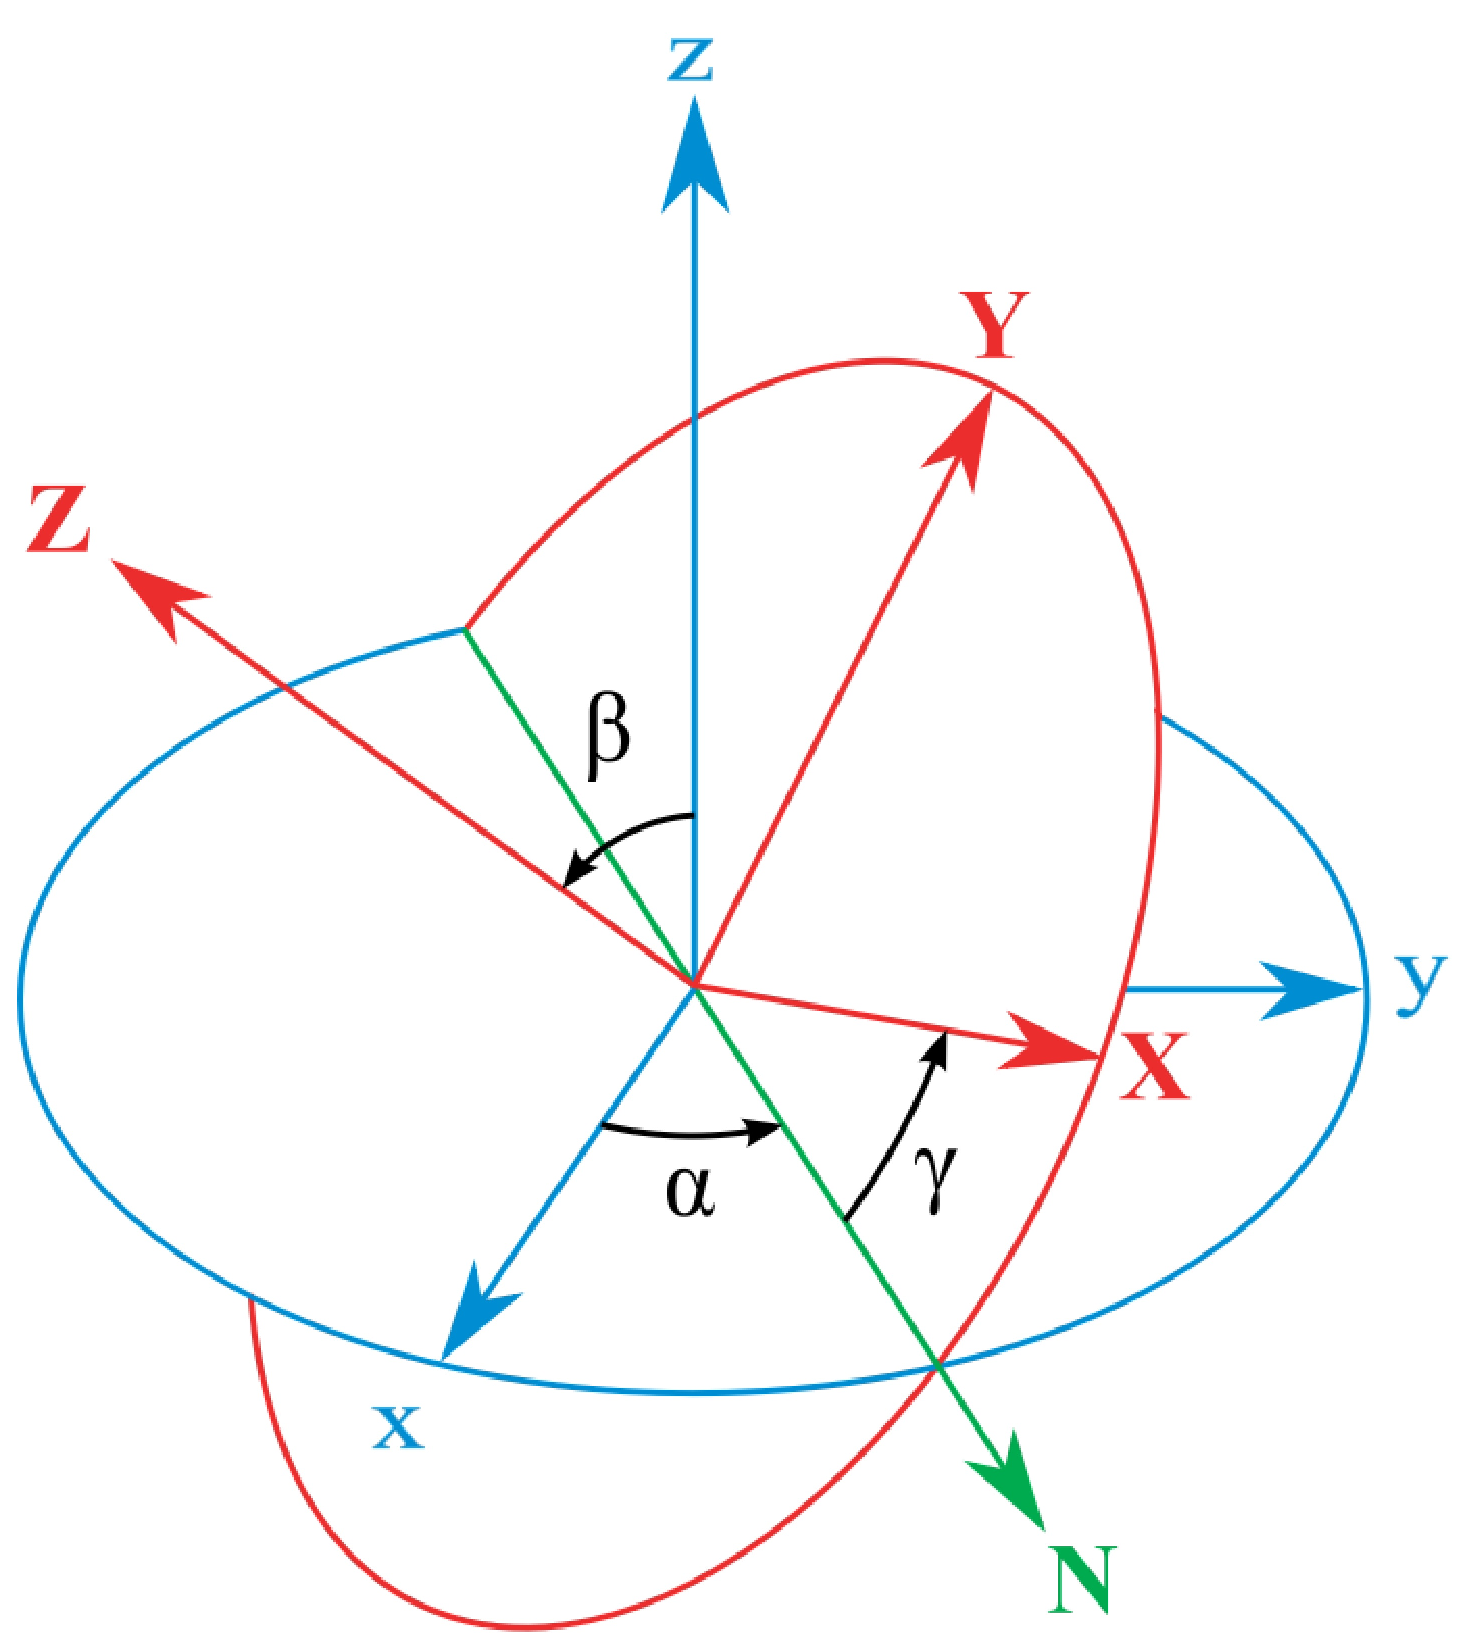
\includegraphics[scale=0.2]{Eulerangles.eps}  \\
    \figurename{ Углы Эйлера}
   \end{center}   
 \end{frame}
 
 \section{Теория}
 
 \begin{frame}{Перспектива} 
   \begin{equation}
    \mathrm{P} =
    \begin{pmatrix}
     \frac{1}{q\tan{\frac{\alpha}{2}}} & 0 & 0 & 0 \\
     0 & \frac{1}{\tan{\frac{\alpha}{2}}}  & 0 & 0\\
     0 & 0 & \frac{-d_n - d_f}{d_n - d_f} & \frac{2d_n d_f}{d_n - d_f}\\
     0 & 0 & 1 & 0
    \end{pmatrix},
   \end{equation}  
 \end{frame}
 
 \section{Заключение}
  
 \begin{frame}{Результаты}
  \begin{itemize}
    \item результат 1
    \item результат 2
  \end{itemize}
 \end{frame} 
 
\end{document}
